\documentclass[nofonts]{ctexart}
%\CTEXsetup[name={Step ,},number={\arabic{chapter}}]{chapter}
\setCJKmainfont[ItalicFont={AR PL UKai CN}]{AR PL UMing CN} %设置中文默认字体
\setCJKsansfont{WenQuanYi Micro Hei} %设置文泉驿正黑字体作为中文无衬线字体
\setCJKmonofont{WenQuanYi Micro Hei Mono} %设置文泉驿等宽正黑字体作为中文打字机字体

\usepackage{amsmath}
%\usepackage{wallpaper}
\usepackage{xcolor}
%\usepackage{pgf, tikz}
\usepackage{multirow}
\usepackage{listings}
\usepackage{color}

\definecolor{keywordcolor}{rgb}{0.8,0.1,0.5}
\definecolor{webgreen}{rgb}{0,.5,0}

%\usepackage[paperwidth=185mm,paperheight=260mm,text={148mm,210mm},left=21mm,includehead,vmarginratio=1:1]{geometry}
%\usepackage[raggedright]{titlesec}
%\titleformat{\chapter}[display]{\Huge\bfseries}{Step \,\thechapter\,}{1em}{}

%\usepackage{fancyhdr}
%\pagestyle{fancy}
%\fancyhf{}
%\fancyhead[ER, OR]{\leftmark}
%\fancyhead[EL, OL]{《编译实习》实习报告}
%\fancyfoot[C]{\thepage}
%\renewcommand{\chaptermark}[1]{\markboth{\thechapter.\ #1}{}}


\lstset{language=C,
basicstyle=\footnotesize,
keywordstyle=\color{keywordcolor}\bfseries, %\underbar,
identifierstyle=,
commentstyle=\color{green} \textit,
stringstyle=\color{red} \ttfamily,
showstringspaces=false,
frame=single,
numbers=left,
numberstyle=\tiny \color{blue},
backgroundcolor=\color{white},
captionpos=b
}


\begin{document}

\title{%
\vspace{-30mm}\Huge NachOS Lab6 实习报告 \vspace{10mm}}
\author{%
\Large 史杨勍惟 
\\[10mm] 1200012741 信息科学技术学院}
\date{2016,06,06}

\maketitle

\newpage
\tableofcontents
\newpage

\section{总体概述}
这次的Lab主要内容是实现文件系统的一些扩展功能。

\section{任务完成列表}
\begin{table}[h]
\footnotesize
\begin{tabular}{|c|c|c|c|c|}\hline
\textbf{Exercise 1} & \textbf{Exercise 2} &
\textbf{Exercise 3} & \textbf{Exercise 4} &
\textbf{Exercise 5}\\\hline
Y & Y & Y & Y & Y\\\hline


\end{tabular}


\end{table}
\section{完成情况}
\subsection*{Exercise 1}
syscall.h 这个头文件声明了所有的系统调用,首先是给每个系统调用设了一个系统调用号,同时定
义了系统调用的模型。所有用户程序都需要 include 这个头文件。
start.s 是一个汇编代码文件,从 test 目录下的 Makefile 文件下可以看出每个用户程序先生成 .o 文
件,然后与 start.o 一起交叉编译为 .coff 文件,最后转换为可执行的 .noff 文件。因此, start.s 相当于一
个系统调用库,当用户程序执行系统调用时会执行对应的 start.s 中的代码。在
start.s 中把对应的系统调用号放入二号寄存器中,然后执行 syscall 汇编语句。这会使得
machine.cc 中的 模拟指令运行函数 OneInstruction 调用 RaiseException 函数,这个函数我们之前
就遇见过,它会调用 exception.cc 中 ExceptionHandler 函数,并且指明 exception 类似为系统调用。
真正系统调用的实现全部在 ExceptionHandler 函数中实现,这也是我们本次 lab 主要完成的部分。
\subsection*{Exercise 2}

Create 系统调用只有一个参数,就是指向文件名的 char 指针。从寄存器 4 可以读出文件名的地址,
特别要注意的是,这个地址是虚拟地址,如果想通过这个地址访问到 char 指针指向的文件名内容,需要
访问 Nachos 的物理内存,这就是 Lab4 的内容了。具体地,从物理内存以字节为单位地读取一个 char 型
变量,直到读完整个文件名,从而知道了文件名的长度。然后再将整个文件名从内存中拷出来,这下就
可以直接调用文件系统中的 Create 函数,新建一个文件,初始化文件大小为 0。
Open 系统调用也是只有一个参数代表文件名,实际上前面的过程和 Create 系统调用实现完全一样,
只不过之后是调用文件系统中的 Open 函数。还有一点要注意的是 Open 系统调用要求返回一个文件描述
符。恰好上个 Lab 已经实现了这一点,因此就直接返回文件的描述符即可。有一张表将文件的描述符和
文件的文件头扇区号,依此扇区号建立一个 OpenFile。
Close 系统调用做的事情很简单,就是回收它的文件描述符。
另一件事情是,上一个 Lab 为了做到文件访问的同步,我维护了一个全局文件链表,其中打开一个
新文件会被加入链表,关闭一个文件会将链表中文件持有线程计数-1。现在,实现了系统调用,觉得应该
把这两个函数分别放到这里,更为合适。
Write 系统调用有三个参数,分别是字符缓存区、写入部分的大小以及要写入的文件的文件描述符。
因为待写入的内容在用户空间,而现在是在内核空间,因此我定义了一个 buffer 将待写入的内容读进来,
这一步需要经过虚实地址的转换。然后通过文件描述符打开文件,类似 Open 函数,再利用 OpenFile 的
Write 方法将内容写入。这里需要额外判断一下,如果文件描述符是 1,即终端,则直接调用 printf,而不
用打开文件了。
Read 系统调用类似 Write 系统调用有三个参数,分别是字符缓冲区、读入部分的大小以及要读入的
文件的文件描述符。这里先判断文件描述符是否为 0,即终端,是的话就调用 scanf 函数等待输入。否则,
还是先打开文件,利用文件系统的 Read 方法将要读出的内容存入一个 buffer 中,然后再将 buffer 的内容
写回到用户空间的相应位置,同样需要经历地址的虚实转换。与 Write 系统调用不同的是,Read 系统调
用还需要返回读出的字节数,这个值放置在寄存器 2 中。
与 Open,Close 一样,上一个 Lab 为了做到文件访问的同步,加入了文件的读写锁,之前是加到了
OpenFile 的 Write 和 Read 里面。现在,实现了系统调用,这两个函数分别放到这里,更为合适。
最后,一个统一的问题是,目前 Nachos 模拟系统调用指令之后不会增加 PC ,这意味着
ExceptionHandler 的相应内容总会被重复执行。为此,需要在每条处理系统调用的分支之后将 PC 加
4 。

\subsection*{Exercise 3}
正好这几个系统调用可以可以完整表征一个文件的声明周期,于是我就都写入一个用户测试程序里
了,系统调用序列是 Create->Open->Write->Read->Close ,具体的,创建名称为 “ Ex3” 的文件,
并写入 “ Good job” 。将这个程序利用 -cp 选项拷贝到 Nachos 的文件系统中,然后运行这个用户测试程
序,运行结果如下:
\begin{figure}[h!]
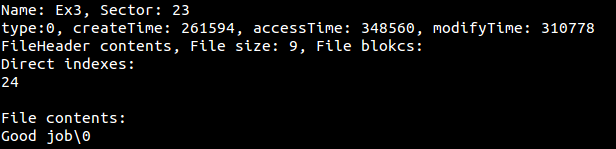
\includegraphics[width=5in]{e31.png}
\end{figure}
可以看到,文件被成功创建,同时查看文件内容,证明写入操作正确。
然后看用户程序输出状况(利用了之前实现的 Print 系统调用)。

\begin{figure}[h!]
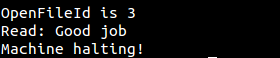
\includegraphics[width=5in]{e32.png}
\end{figure}
可以看到, Open 文件返回文件描述符 3 ( 0,1,2, 预留,虽然 Nachos 似乎并没有 2...... )。
中间两行是文件系统的输出,忽略。
倒数第二行显示了读出的内容,是正确的。


\subsection*{Exercise 4}
Exec 系统调用有一个参数,表示可执行文件的文件名。这个系统调用让一个新线程去运行这个可执
行文件。其实这有点像我们在 Lab4 中让多个线程运行用户程序的步骤,实际上我也是基本上把上次的
实现搬到这里来了。首先还是先通过文件名打开对应的可执行文件,然后新建一个线程,初始化它的用
户空间,设置它对应的内存交换文件(用于 lazy-loading ,在 Lab4 实现)。然后,令新线程调用 Fork
执行一个函数,在这个函数中进行机器页表和寄存器的切换,再调用 machine->Run 方法执行用户程序。
此系统调用需要返回标识一个用户空间的 SpaceId ,我觉得因为一个线程就是对应的一个用户空间,因
此我就直接返回新线程的 tid 了。
Fork 系统调用有一个参数,表示新 fork 出来的线程去执行的函数。这个系统调用与 Exec 不同,要
求新 fork 的线程与原来的线程拥有相同的用户空间内容。为此,我给 AddrSpace 类添加了一个新的构
造函数,接收参数不再是一个可执行文件,而是一个 AddrSpace 的指针,代表父线程的用户空间。最
主要的事情,就是将父线程用户空间对应的交换文件拷贝到子线程地址空间中,具体地,利用文件系统
的 Read 方法读出内容,再用 Write 方法写到新文件中。这里特别要注意的是,父线程此时可能还有未
写回的部分,所以此时必须全部写回从而正确地记录父线程用户空间的状态。之后,还要注意调用
Thread 类的 SaveUserState 函数将父线程的全部寄存器保存。由于要求子线程下一步去执行 func 函
数,因此在这里设置 PC 寄存器和 NextPC 寄存器,让它们分别指向 func 的地址以及 func 地址 +4 。最
后,然后。令新线程调用 Fork 执行一个函数,在这个函数中进行机器页表和寄存器的切换,再调用
machine->Run 方法执行继续用户程序。
Yield 系统调用直接让 currentThread 执行 Thread 类的 Yield 方法。
Join 系统调用有一个参数,表示当前线程需要等待该线程 ID 的线程运行完毕再运行。为此,我给
Thread 类定义了一个静态变量 JoinTable ,记录有关 Join 操作的相关信息。它实际是一个 map , key
是线程 id , value 是一个 List 指针,直线的链表里是等待该线程的所有线程的实例( Thread* )。同时
还在 Thread 下添加两个方法。一个方法是将自己加入到某线程的等待队列中,具体是从 JoinTable 中
找到该队列然后把自己加入队列,如果没有队列则新建一个。另一个方法是将某线程的等待队列中的线
程全部唤醒,实际上就是执行 ReadyToRun 。这个方法在 Thread 类的 Finish 中被调用,此时意味着
该线程已经结束了,因此可以唤醒等待的线程。有了这些辅助, Join 系统调用时很好写,就是将当前线
程加入对应线程 ID 的等待队列中,然后关闭中断,自己调用 Sleep 。等待唤醒后,再恢复中断到原来状
态。
Exit 系统调用直接让 currentThread 执行 Thread 类的 Finish 方法,当然同时应该记录退出码用
于检测错误。

\subsection*{Exercise 5}
测试代码1:
\begin{lstlisting}
int tid;
int code = 0;
tid = Exec("sort");
Join(tid);
Join(code);
\end{lstlisting}

理想情况下,新线程去执行 sort 用户程序(这个用户程序被我修改,功能是排序 16 个数,并且在
最后打印数组), main 线程需要等待到这个线程运行结束,再退出。运行结果如下:
\begin{figure}[h!]
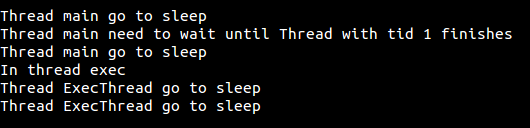
\includegraphics[width=5in]{e651.png}
\end{figure}

首先,当 Exec 系统调用被执行时,新线程 ExecThread 被创建。当 Join 系统调用被执行时,
main 线程 sleep (第 80 行), ExecThread 被调度。

\begin{figure}[h!]
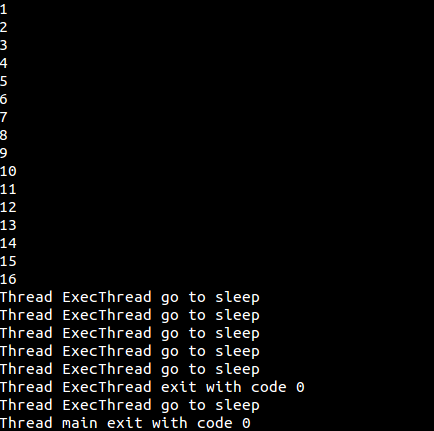
\includegraphics[width=5in]{e652.png}
\end{figure}

最终, ExecThread 正确运行 sort 用户程序,打印出了 16 个正确顺序的数字,同时先退出(第
138 行),结束运行。 main 这时才被激活退出(第 140 行)。
再测试 Fork 和 Yield 。具体如下:

测试代码1:
\begin{lstlisting}
int val = 1;
void func()
{ 
	Exit(val);
}

int main() 
{
	val++;
	Fork(func);
	Yield();
	val++;
	Exit(val);
\end{lstlisting}

理想情况下, main 线程的退出码是 3 (做了两次自加),而 fork 线程的退出码是 2 (只做了最开始
的一次自加)。

测试结果正确。


\section{遇到的困难以及解决办法}
无

\section{收获与感想}
终于完成了最后一个Lab,这学期作为大四的学生水过了所有的Lab。

个人觉得我完成的质量很不好,当初大三是因为第一次小测觉得分数太低所以果断退课了,现在发现到了大四,已经没有当初的鸿鹄之志,一心只想水过任务了。其实操作系统实习尤其是这个Nachos是很有意思的一个项目,在各种的地方都可以发挥个性化的实现方式。不过的确也还是需要时间的,毕竟这种底层的系统调试起来容易身心疲惫,当然,这或许也是程序员的必修技能吧。

说实话,在完成过程中,我前3个Lab参照了自己去年的实现,后3个Lab参照了去年队友的实现,不过自己把这些代码复现了一遍。我很惭愧自己完成的不好,没有很花时间,也给助教添了不少麻烦。感谢今年助教和陈老师耐心的讲解。当然也希望助教给分的时候手下留情,能给我及格就好啦~如果以后有机会,我一定会好好把Nachos重头开始在做一遍!



\section{意见与建议}
无。

\section{参考资料}
\begin{itemize}
\item 《现代操作系统》
\end{itemize}

\end{document}